% !TeX spellcheck = en_US
\addscenariosection{1}{Clash/Alliance Scenario}{The Shattered Alliance}{\images/implosion.png}

\begin{multicols*}{2}

\textbf{Author:} LAAMAKALA

\textit{Once united, the great kingdoms of Aldara now stand divided. Betrayal and ambition fuel the conflict — who will forge a new order?}  % no-check-caps

\subsection*{\MakeUppercase{Scenario Length}}
This Scenario plays out over 14 Rounds.

\subsection*{\MakeUppercase{Player Setup}}
\textbf{Player Count:} 3 or 6P FFA, 2v2v2 alliance.

\textbf{Starting Resources:} 14 \svg{gold}, 4 \svg{building_materials}, 1 \svg{valuables}

\textbf{Starting Income:} 10 \svg{gold}, 0 \svg{building_materials}, 0 \svg{valuables}

\textbf{Starting Units:}

\begin{itemize}
  \item 2 × Few cheapest \svg{bronze} Units
\end{itemize}

\textbf{Town Buildings:}
\begin{itemize}
  \item \bronze\ Dwelling
\end{itemize}

\subsection*{\MakeUppercase{Map Setup}}
Take the following Map Tiles and arrange them as shown in the Scenario map layout:

\begin{itemize}
  \item 6 × Starting (I) Map Tiles
  \item 3 × Far (II-III) Map Tiles for each player's Map Pool
  \item 12 × Near (IV-V) Map Tiles
  \item 3 × Center (VI-VII) Map Tiles
\end{itemize}

\subsection*{\MakeUppercase{Victory Conditions}}
The game ends when one player has defeated each other players' Main Hero once \textit{or} at the end of Round 14.

\subsection*{\MakeUppercase{Victory Points}}
The player with the most Victory Points (VP) wins (see Tournament Book). Players gain:

\begin{itemize}
  \item 1 VP for losing a Combat against another player
  \item 1 VP for each Starting Town captured - \textit{once per captured Faction}
  \item 1 VP for the Grail Token
  \item 2 VP for winning a Level VII Neutral Combat
  \item 1 VP for every controlled Mine or Settlement on Near and Center Tiles
  \item Removed Artifacts count towards VPs
\end{itemize}

\subsection*{\MakeUppercase{Timed Events}}

\begin{itemize}
  \item[\textbf{\nth{1}}] \textbf{Round:} Each player may build the \svg{building_special_tent} building with a discount of 4 \svg{gold} and 2 \svg{building_materials}.
  \item[\textbf{\nth{2}}] \textbf{Round:} Each player may gain one reward from the Field the closest player to them visits this Round.
  \item[\textbf{\nth{4}}] \textbf{Round:} Remove all Black Cubes.
  \item[\textbf{\nth{6}}] \textbf{Round:} Secondary Heroes gain +1 \svgeven{movement}.
  \item[\textbf{\nth{8}}] \textbf{Round:} Each player may remove up to 5 Black Cubes from the map.
  \item[\textbf{\nth{9}}] \textbf{Round:} Player(s) whose Main Hero has the least \svg{experience}, roll 2 \svg{resource}.
  \item[\textbf{\nth{10}}] \textbf{Round:} All players may recruit a Secondary Hero for free.
  \item[\textbf{\nth{11}}] \textbf{Round:} Remove all Black Cubes.
  \item[\textbf{\nth{12}}] \textbf{Round:} Each player may recruit one \silver\ Neutral Unit from the closest player's Faction for half its recruitment cost.
\end{itemize}

\subsection*{\MakeUppercase{Additional Rules}}
\begin{itemize}
  \item \textbf{Sanctuary:} Choose 1 \svg{spellpower} from your M\&M Deck and add it to your hand, then reshuffle your Deck. \textit{Visitable once per Faction.}
  \item \textbf{Obelisk:} Choose 1 \svg{artifact} from your M\&M Deck and add it to your hand, then reshuffle your Deck. \textit{Visitable once per Faction.}
  \item \textbf{Dragon Utopia:} Defended only by Dragons. Recruit one Neutral Dragon you defeated for half its recruitment cost (rounded up).
  \item \textbf{Random Town:} On next Resource Round, you may recruit one random Neutral \silver\ Unit by paying its full \svg{pay_v2} cost.
  \item \textbf{Grail Field:} Gain the Grail Token.
  \item If you start a turn with the Grail Token, gain +1 \svg{morale_positive} \textit{and} 5 \svg{gold}. If a Hero with the Grail Token is defeated, the Grail Token is given to the winner of that Combat.
  \item If a Hero with the Grail Token uses Dimension Door, Fly, or Town Portal, the Grail Token is dropped on the origin Field before the Hero moves.
  \item \textbf{Level VII Settlement:} You may Reinforce \textbf{and} increase income.
  \item Level VII Neutral Combats cannot be skipped and grant the player +1 \svg{morale_positive}.
\item Players do not have to pay \svg{gold} after losing a Combat against another player.
  \item A defeated Main Hero may Empower one Statistic Card from their M\&M Deck \textit{and} gain +1 \svg{morale_positive}.
  \item With fewer than 6 players, Starting Towns of unused Factions are defended similarly to a Random Town.
  \item Flagging a Neutral Starting Town increases two incomes by 1 space.
\end{itemize}

\begin{center}
  \vspace*{\fill}
  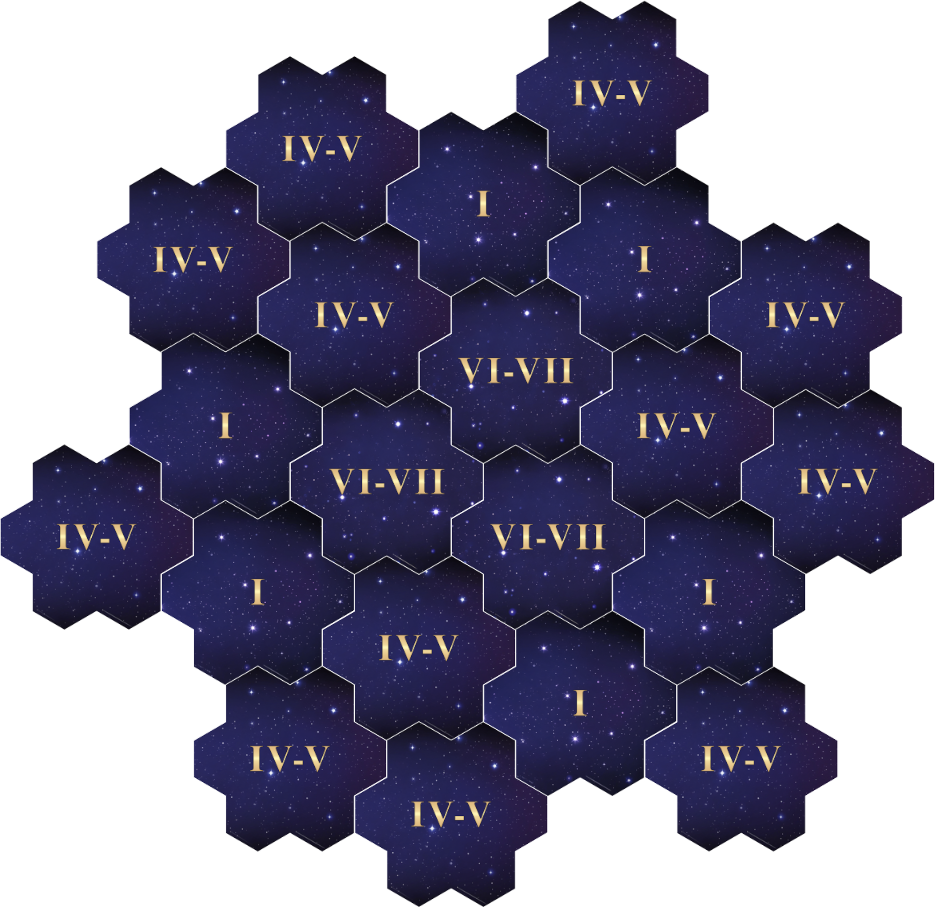
\includegraphics[width=1.0\linewidth]{\maps/shattered_alliance-6p.png}
  \captionof{figure}{\textbf{SCENARIO MAP LAYOUT}}
  \vspace*{\fill}
  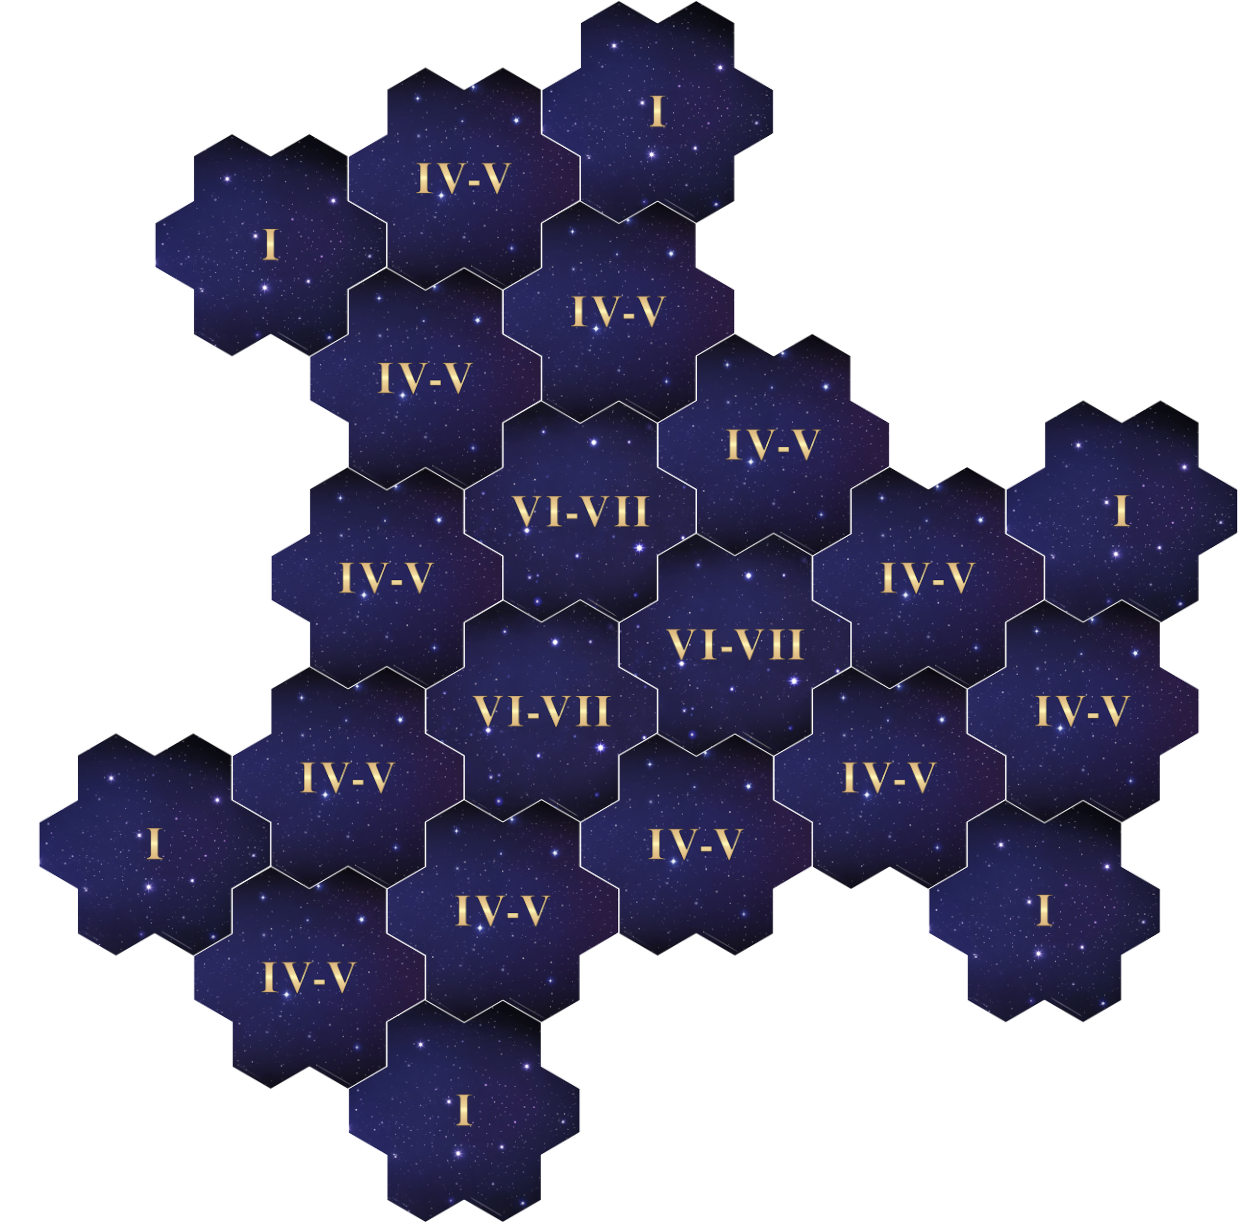
\includegraphics[width=1.1\linewidth]{\maps/shattered_alliance_alt-6p.png}
  \captionof{figure}{\textbf{ALTERNATIVE MAP LAYOUT}}
  \vspace*{\fill}
\end{center}

\end{multicols*}
